\chapter{Keko}

Keko on tietorakenne, joka pitää yllä alkioiden kokoelmaa
ja tarjoaa seuraavat operaatiot:

\begin{itemize}
\item lisää alkio $x$ joukkoon
\item etsi joukon pienin/suurin alkio
\item poista joukon pienin/suurin alkio
\end{itemize}

Keon toiminta riippuu siitä, onko kyseessä minimikeko
vai maksimikeko.
Minimikeossa voimme etsiä ja poistaa pienimmän alkion,
kun taas maksimikeossa voimme etsiä ja poistaa suurimman alkion.
Meidän täytyy päättää keon luontivaiheessa,
onko keko minimikeko vai maksimikeko.

Tässä luvussa tutustumme binäärikeko-rakenteeseen,
jossa lisäykset ja poistot vievät aikaa $O(\log n)$
ja haku vie aikaa $O(1)$.
Binäärikeko toteutetaan binääripuun avulla,
ja se on tavallisimmin käytetty kekorakenne.
Javan standardikirjaston tietorakenne prioriteettijono
perustuu binäärikekoon.

\section{Binäärikeko}

\emph{Binäärikeko} on binääripuu, jonka jokaisessa solmussa on
yksi kokoelmaan kuuluva alkio.
Puu on rakennettu niin, että sen kaikki tasot alinta
tasoa lukuun ottamatta ovat täynnä solmuja,
eli kaikilla solmuilla on vasen ja oikea lapsi.
Alin taso on puolestaan täytetty niin,
että solmut on sijoitettu mahdollisimman vasemmalle
ylempien solmujen lapsiksi.

Binäärikeon toiminta perustuu siihen,
että jokainen keon solmu täyttää \emph{kekoehdon}.
Minimikeossa kekoehto vaatii, että jokaisen
solmun arvo on suurempi tai yhtä suuri kuin solmun vanhemman arvo.
Maksimikeossa puolestaan jokaisen solmun arvon tulee olla
pienempi tai yhtä suuri kuin solmun vanhemman arvon.
Kekoehdon ansiosta minimikeon juuressa on kokoelman
pienin alkio ja maksimikeon juuressa on kokoelman suurin alkio.

\begin{figure}
\center
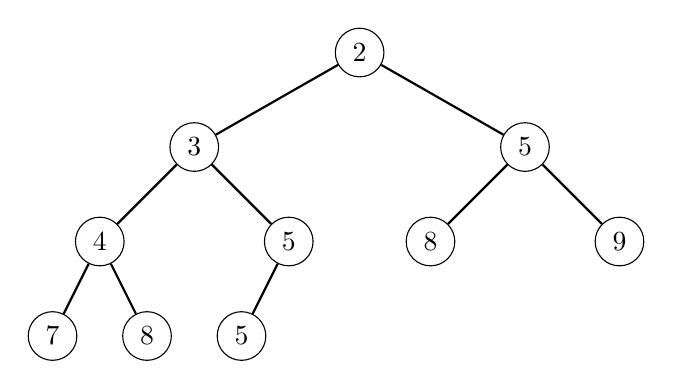
\begin{tikzpicture}[scale=0.6]
\node[draw, circle] (1) at (0,0) {$2$};
\node[draw, circle] (2) at (-3.5,-2) {$3$};
\node[draw, circle] (3) at (3.5,-2) {$5$};
\node[draw, circle] (4) at (-5.5,-4) {$4$};
\node[draw, circle] (5) at (-1.5,-4) {$5$};
\node[draw, circle] (6) at (1.5,-4) {$8$};
\node[draw, circle] (7) at (5.5,-4) {$9$};
\node[draw, circle] (8) at (-6.5,-6) {$7$};
\node[draw, circle] (9) at (-4.5,-6) {$8$};
\node[draw, circle] (10) at (-2.5,-6) {$5$};
\path[draw,thick,-] (1) -- (2);
\path[draw,thick,-] (1) -- (3);
\path[draw,thick,-] (2) -- (4);
\path[draw,thick,-] (2) -- (5);
\path[draw,thick,-] (3) -- (6);
\path[draw,thick,-] (3) -- (7);
\path[draw,thick,-] (4) -- (8);
\path[draw,thick,-] (4) -- (9);
\path[draw,thick,-] (5) -- (10);
\end{tikzpicture}
\caption{Minimikeko, joka vastaa kokoelmaa $[2,3,4,5,5,5,7,8,8,9]$.}
\label{fig:minkek}
\end{figure}


Kuvassa \ref{fig:minkek} on esimerkkinä minimikeko,
johon on tallennettu kymmenen alkiota.
Keon kolme ensimmäistä kerrosta ovat täynnä
ja neljännessä kerroksessa kolme ensimmäistä kohtaa on käytetty.
Keon juurena on kokoelman pienin alkio $2$,
ja kaikki solmut täyttävät kekoehdon.
Huomaa, että sama alkio voi esiintyä keossa useasti,
kuten tässä keossa alkiot $5$ ja $8$.

\subsection{Keon tallentaminen}

Tallennamme binäärikeon \emph{taulukkona},
joka sisältää keon solmujen arvot jär\-jestyksessä
ylhäältä alaspäin ja vasemmalta oikealle.
Tämä tehokas tallennustapa on mahdollinen,
koska keon kaikki tasot ovat täynnä solmuja.
Tallennamme keon taulukkoon kohdasta $1$ alkaen,
koska tämä helpottaa keon operaatioiden toteuttamista.

Esimerkiksi tallennamme kuvan \ref{fig:minkek}
keon taulukkona seuraavasti:

\begin{code}
int[] keko = {0,2,3,5,4,5,8,9,7,8,5};
\end{code}

Huomaa, että taulukon ensimmäinen alkio on $0$,
koska emme käytä kohtaa $0$ keon tallentamiseen.

Tämän tallennustavan etuna on, että voimme laskea
helposti, missä kohdissa keon alkiot ovat taulukossa.
Ensinnäkin keon juuri eli pienin tai suurin alkio
on aina kohdassa $1$.
Lisäksi jos tiedämme, että tietty solmu on kohdassa $k$,
niin tästä seuraa, että

\begin{itemize}
\item solmun vasen lapsi on kohdassa $2k$,
\item solmun oikea lapsi on kohdassa $2k+1$ ja
\item solmun vanhempi on kohdassa $\lfloor k/2 \rfloor$.
\end{itemize}

Esimerkissämme solmu 4
on taulukossa kohdassa $4$,
joten sen lapset ovat kohdissa $8$ ja $9$
ja sen vanhempi on kohdassa $2$.

\subsection{Operaatioiden toteutus}

\subsection{Operaatiot}

Meidän on helppoa etsiä minimikeon pienin alkio $O(1)$-ajassa,
koska se on aina keon juuressa.
Seuraavaksi näemme, kuinka voimme toteuttaa alkion lisäämisen
sekä pienimmän alkion poistamisen $O(\log n)$-ajassa.

\subsubsection{Alkion lisääminen}

Kun lisäämme uuden alkion kekoon, lisäämme sen ensin seuraavaan
vapaana olevaan paikkaan. Jos alimmalla kerroksella on tilaa,
lisäämme sen sinne mahdollisimman vasemmalle,
ja muuten aloitamme uuden kerroksen, jossa on vain uusi solmu.

Alkion lisäämisen jälkeen meidän täytyy varmistaa,
että kekoehto säilyy edelleen voimassa.
Tämä tapahtuu siirtämällä alkiota ylöspäin keossa
niin kauan kuin se on vanhempaansa pienempi.
Koska täytämme kekoa tasaisesti, sen korkeus on $O(\log n)$
ja operaatio toimii $O(\log n)$-ajassa.

\begin{figure}
\center
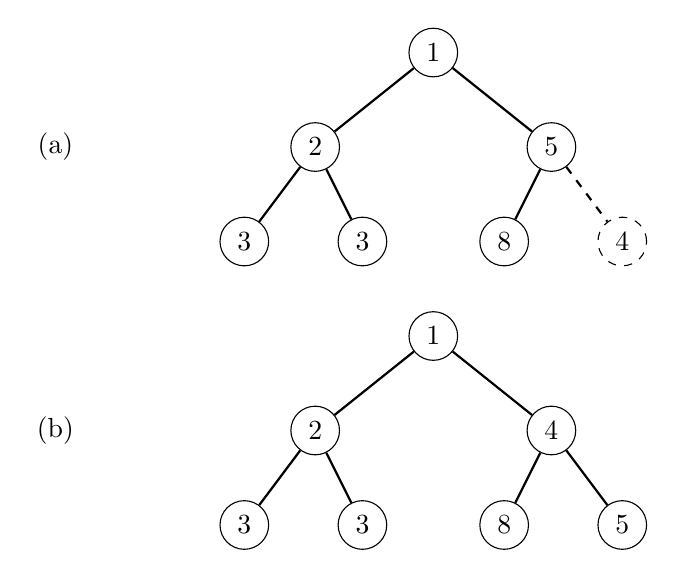
\begin{tikzpicture}[scale=0.6]
\begin{scope}
\node at (-8,-2) {(a)};
\node[draw, circle] (1) at (0,0) {$1$};
\node[draw, circle] (2) at (-2.5,-2) {$2$};
\node[draw, circle] (3) at (2.5,-2) {$5$};
\node[draw, circle] (4) at (-4,-4) {$3$};
\node[draw, circle] (5) at (-1.5,-4) {$3$};
\node[draw, circle] (6) at (1.5,-4) {$8$};
\node[draw, circle, dashed] (7) at (4,-4) {$4$};
\path[draw,thick,-] (1) -- (2);
\path[draw,thick,-] (1) -- (3);
\path[draw,thick,-] (2) -- (4);
\path[draw,thick,-] (2) -- (5);
\path[draw,thick,-] (3) -- (6);
\path[draw,thick,-,dashed] (3) -- (7);
\end{scope}
\begin{scope}[yshift=-6cm]
\node at (-8,-2) {(b)};
\node[draw, circle] (1) at (0,0) {$1$};
\node[draw, circle] (2) at (-2.5,-2) {$2$};
\node[draw, circle] (3) at (2.5,-2) {$4$};
\node[draw, circle] (4) at (-4,-4) {$3$};
\node[draw, circle] (5) at (-1.5,-4) {$3$};
\node[draw, circle] (6) at (1.5,-4) {$8$};
\node[draw, circle] (7) at (4,-4) {$5$};
\path[draw,thick,-] (1) -- (2);
\path[draw,thick,-] (1) -- (3);
\path[draw,thick,-] (2) -- (4);
\path[draw,thick,-] (2) -- (5);
\path[draw,thick,-] (3) -- (6);
\path[draw,thick,-] (3) -- (7);
\end{scope}
\end{tikzpicture}
\caption{Alkion 4 lisääminen kekoon. (a) Lisäämme alkion ensimmäiseen
vapaana olevaan paikkaan. (b) Koska alkio on vanhempaansa pienempi,
vaihdamme alkiot keskenään.}
\label{fig:keklis}
\end{figure}

Kuva \ref{fig:keklis} näyttää esimerkin alkion lisäämisestä kekoon.
Lisäämme ensin alkion 4 keon ensimmäiseen vapaana olevaan paikkaan.
Koska uuden solmun arvo on sen vanhemman arvoa pienempi,
vaihdamme nämä arvot keskenään. Tämän jälkeen kekoehto on voimassa.

\subsubsection{Pienimmän alkion poistaminen}

Kun haluamme poistaa keon pienimmän alkion, vaihdamme ensin keskenään
juuressa olevan pienimmän arvon sekä keon viimeisessä käytössä olevassa
paikassa olevan arvon. Tämän jälkeen poistamme keon viimeisen solmun,
jolloin pienin arvo katoaa keosta.

Tämän jälkeen meidän täytyy jälleen huolehtia siitä, että kekoehto pätee.
Tämä tapahtuu laskettamalla juuressa olevaa arvoa alaspäin keossa,
kunnes kekoehto pätee. Valitsemme aina kahdesta mahdollisesta suunnasta sen,
jossa on pienempi alkio.
Koska alkio laskeutuu enintään $O(\log n)$ askelta,
tämäkin operaatio toimii ajassa $O(\log n)$.

\begin{figure}
\center
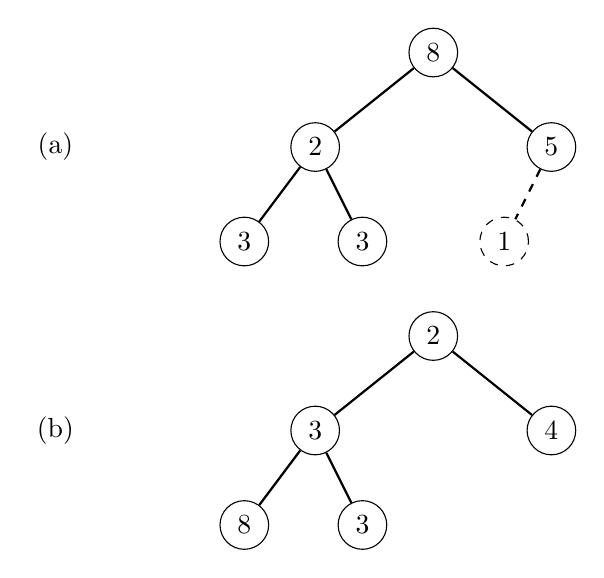
\begin{tikzpicture}[scale=0.6]
\begin{scope}
\node at (-8,-2) {(a)};
\node[draw, circle] (1) at (0,0) {$8$};
\node[draw, circle] (2) at (-2.5,-2) {$2$};
\node[draw, circle] (3) at (2.5,-2) {$5$};
\node[draw, circle] (4) at (-4,-4) {$3$};
\node[draw, circle] (5) at (-1.5,-4) {$3$};
\node[draw, circle, dashed] (6) at (1.5,-4) {$1$};
\path[draw,thick,-] (1) -- (2);
\path[draw,thick,-] (1) -- (3);
\path[draw,thick,-] (2) -- (4);
\path[draw,thick,-] (2) -- (5);
\path[draw,thick,-,dashed] (3) -- (6);
\end{scope}
\begin{scope}[yshift=-6cm]
\node at (-8,-2) {(b)};
\node[draw, circle] (1) at (0,0) {$2$};
\node[draw, circle] (2) at (-2.5,-2) {$3$};
\node[draw, circle] (3) at (2.5,-2) {$4$};
\node[draw, circle] (4) at (-4,-4) {$8$};
\node[draw, circle] (5) at (-1.5,-4) {$3$};
\path[draw,thick,-] (1) -- (2);
\path[draw,thick,-] (1) -- (3);
\path[draw,thick,-] (2) -- (4);
\path[draw,thick,-] (2) -- (5);
\end{scope}
\end{tikzpicture}
\caption{Pienimmän alkion poistaminen keosta. (a) Vaihdamme keskenään
pienimmän alkion ja viimeisen alkion. (b) Alkio 8 laskeutuu keon
huipulta takaisin sen pohjalle.}
\label{fig:kekpoi}
\end{figure}

Kuva \ref{fig:kekpoi} näyttää esimerkin alkion poistamisesta keosta.
Aluksi vaihdamme keskenään keon pienimmän alkion $1$
ja viimeisenä keossa olevan alkion $8$.
Tämän jälkeen lasketamme alkiota $8$ juuresta alaspäin,
kunnes kekoehto on voimassa.
Tässä tapauksessa alkio laskeutuu keon pohjalle asti.

\subsection{Toteutus taulukkona}

Kätevä tapa toteuttaa keko on tallentaa sen solmujen
sisältö taulukkoon järjestyksessä ylhäältä alas ja vasemmalta oikealle.
Jotta voimme toteuttaa mukavasti keon operaatiot,
käytämme 1-indeksoitua taulukkoa.
Kuva \ref{fig:kektau} näyttää esimerkin keon tallentamisesta taulukkoon.

\begin{figure}
\center
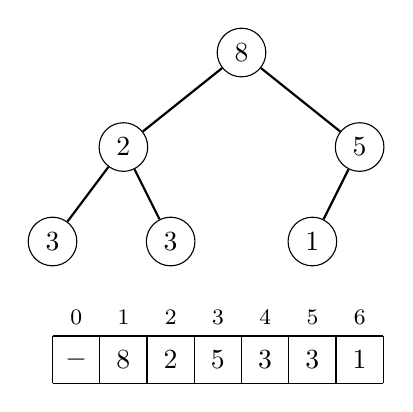
\begin{tikzpicture}[scale=0.6]
\begin{scope}
\node[draw, circle] (1) at (0,0) {$8$};
\node[draw, circle] (2) at (-2.5,-2) {$2$};
\node[draw, circle] (3) at (2.5,-2) {$5$};
\node[draw, circle] (4) at (-4,-4) {$3$};
\node[draw, circle] (5) at (-1.5,-4) {$3$};
\node[draw, circle] (6) at (1.5,-4) {$1$};
\path[draw,thick,-] (1) -- (2);
\path[draw,thick,-] (1) -- (3);
\path[draw,thick,-] (2) -- (4);
\path[draw,thick,-] (2) -- (5);
\path[draw,thick,-] (3) -- (6);
\end{scope}
\begin{scope}[yshift=-7cm,xshift=-4cm]
\draw (0,0) grid (7,1);
\node at (0.5,0.5) {$-$};
\node at (1.5,0.5) {$8$};
\node at (2.5,0.5) {$2$};
\node at (3.5,0.5) {$5$};
\node at (4.5,0.5) {$3$};
\node at (5.5,0.5) {$3$};
\node at (6.5,0.5) {$1$};
\footnotesize
\node at (0.5,1.4) {$0$};
\node at (1.5,1.4) {$1$};
\node at (2.5,1.4) {$2$};
\node at (3.5,1.4) {$3$};
\node at (4.5,1.4) {$4$};
\node at (5.5,1.4) {$5$};
\node at (6.5,1.4) {$6$};
\end{scope}
\end{tikzpicture}
\caption{Keko ja sen taulukkoesitys.}
\label{fig:kektau}
\end{figure}

Kun meillä on tiedossa solmun kohta taulukossa,
voimme helposti selvittää sen lasten ja vanhemman kohdat.
Kohdassa $k$ olevan solmun vasen lapsi on kohdassa $2k$
ja oikea lapsi on kohdassa $2k+1$.
Lisäksi solmun vanhempi on kohdassa $\lfloor k/2 \rfloor$.
Tämän ansiosta voimme toteuttaa keon operaatiot niin,
että niiden vakiokertoimet ovat pienet.

\subsection{Tehokas luonti}

Suoraviivainen tapa luoda $n$ alkiota sisältävä keko
on lisätä jokainen alkio erikseen kekoon $O(\log n)$-ajassa.
Tällä tavalla saamme rakennettua keon $O(n \log n)$-ajassa.
Osoittautuu kuitenkin, että keon luominen taulukon pohjalta
on mahdollista myös $O(n)$-ajassa.

Ideana on käydä läpi keon solmut lopusta alkuun ja
jokaisen solmun kohdalla varmistaa,
että siitä solmusta alkava alipuu toteuttaa kekoehdon
laskettamalla solmun juuressa olevaa arvoa alaspäin.
Kun olemme lopulta käsitelleet kaikki solmut juureen asti,
koko taulukko toteuttaa kekoehdon.

Miksi sitten tämä vie aikaa vain $O(n)$?
Oletetaan, että keossa on $h$ kerrosta ja kaikki
kerrokset ovat täynnä solmuja, eli siinä on $n=2^h-1$ solmua.
Laskemme jokaiselle kerrokselle, montako arvoa laskeutuu
enintään jostakin tämän kerroksen solmusta alaspäin. Tästä saamme:

\begin{itemize}
\item Kerroksesta 1 kerrokseen 2 laskeutuu enintään 1 arvo.
\item Kerroksesta 2 kerrokseen 3 laskeutuu enintään $1+2$ arvoa.
\item Kerroksesta 3 kerrokseen 4 laskeutuu enintään $1+2+4$ arvoa.
\item Jne.
\end{itemize}

Yleisemmin kerroksesta $k$ kerrokseen $k+1$ laskeutuu
enintään $1+2+\dots+2^{k-1} = 2^k-1$ arvoa.
Koska kerroksia on $h$ ja viimeisestä kerroksesta ei voi laskeutua alaspäin,
kokonaistyömäärä on enintään
\[(2^1-1)+(2^2-1)+\dots+(2^{h-1}-1)=2^h-h \le n,\]
joten aikaa kuluu vain $O(n)$.

\subsection{Kekojärjestäminen}

\section{Prioriteettijono}

Monissa ohjelmointikielissä kekoa vastaava tietorakenne
tunnetaan nimellä prioriteettijono.
Näin on myös Javassa, jonka standardikirjastoon 
kuuluu tietorakenne \texttt{PriorityQueue}.
Se on binäärikekoon perustuva tietorakenne,
joka toteuttaa oletuksena minimikeon.

Seuraava koodi esittelee Javan prioriteettijonon toimintaa.
Metodi \texttt{add} lisää alkion jonoon,
metodi \texttt{peek} hakee pienimmän alkion
ja metodi \texttt{poll} hakee ja poistaa pienimmän alkion.

\begin{code}
PriorityQueue<Integer> jono = new PriorityQueue<>();
jono.add(5);
jono.add(3);
jono.add(8);
jono.add(7);
System.out.println(jono.peek()); // 3
System.out.println(jono.poll()); // 3
System.out.println(jono.poll()); // 5
\end{code}

Jos haluamme luoda prioriteettijonon, joka toimiikin
maksimikekona, voimme tehdä sen seuraavaan tapaan:

\begin{code}
PriorityQueue<Integer> jono =
    new PriorityQueue<>(10,Collections.reverseOrder());
\end{code}

Tässä tilanteessa meidän täytyy antaa konstruktorille kaksi tietoa:
rakenteelle alussa varattava tila (tässä 10)
sekä alkioiden järjestämistapa (tässä käänteinen järjestys).

\section{Tehokkuusvertailu}

Keon käyttämisestä voi olla hyötyä binäärihakupuuhun verrattuna,
jos meille riittää, että voimme etsiä ja poistaa pienimmän/suurimman alkion
joukosta.
Seuraavaksi selvitämme, millainen Javan rakenteilla
\texttt{PriorityQueue} ja \texttt{TreeSet} on käytännössä.

Testissämme järjestämme luvut $1,2,\dots,n$ ensin satunnaiseen järjestykseen.
Tämän jälkeen lisäämme puolet luvuista joukkoon
ja sitten toistuvasti lisäämme uuden luvun joukkoon
ja poistamme joukosta pienimmän alkion.
Samalla laskemme joukosta poistettujen alkioiden summan.

Käytämme seuraavaa koodia mittaamaan \texttt{PriorityQueue}-rakenteen tehokkuutta:

\begin{code}
long summa(int[] luvut) {
    PriorityQueue<Integer> jono = new PriorityQueue<>();
    for (int i = 0; i < n/2; i++) {
        jono.add(luvut[i]);
    }
    long summa = 0;
    for (int i = n/2; i < n; i++) {
        jono.add(luvut[i]);
        summa += jono.poll();
    }
    return summa;
}
\end{code}

Vastaavasti käytämme seuraavaa koodia mittaamaan \texttt{TreeSet}-rakenteen tehokkuutta:

\begin{code}
long summa(int[] luvut) {
    TreeSet<Integer> joukko = new TreeSet<>();
    for (int i = 0; i < n/2; i++) {
        joukko.add(luvut[i]);
    }
    long summa = 0;
    for (int i = n/2; i < n; i++) {
        joukko.add(luvut[i]);
        summa += jono.pollFirst();
    }
    return summa;
}
\end{code}

Taulukko \ref{tab:kekver} sisältää vertailun tulokset.
Tässä testissä \texttt{PriorityQueue} toimii 2–3
kertaa nopeammin kuin \texttt{TreeSet},
eli sen käyttämisestä on perusteltua hyötyä.

\begin{table}
\center
\begin{tabular}{rrrr}
taulukon koko $n$ & \texttt{PriorityQueue} & \texttt{TreeSet} \\
\hline
$10^6$ & 0.29 s & 0.78 s \\
$2 \cdot 10^6$ & 0.71 s & 1.50 s \\
$4 \cdot 10^6$ & 1.56 s & 3.72 s \\
$8 \cdot 10^6$ & 3.68 s & 9.43 s \\
\end{tabular}
\caption{Algoritmien suoritusaikojen vertailu.}
\label{tab:kekver}
\end{table}